\icode{E-EME-SI-L3-261121-001}
如图所示，两个带有同种电荷的小球，用绝缘细线悬挂于\(O\)点，若\(q_1> q_2\)，\(L_1 >L_2\)，平衡时两球到过\(O\)点的竖直线的距离相等，则根据三角形相似关系，可得\paren[]
	
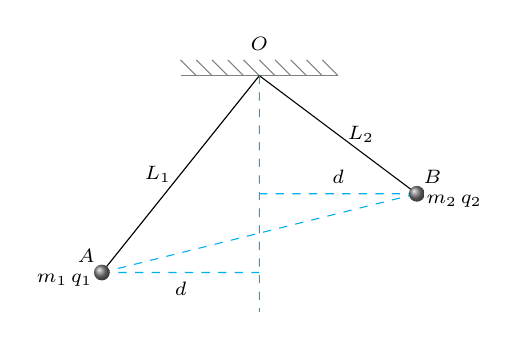
\begin{tikzpicture}[>=stealth,font=\scriptsize]
	\draw[gray] (-1,0)--(1,0);
	\foreach \x in {-1,-.8,...,.8}
		\draw[gray] (\x,.2)--++(.2,-.2);
	\draw(0,0)--node[left]{\(L_1\)}(-2,-2.5) (0,0)--node[right]{\(L_2\)}(2,-1.5);
	\draw[dashed,cyan] (-2,-2.5)--(2,-1.5) (0,0)--(0,-3) (-2,-2.5)--node[below,black]{\(d\)}(0,-2.5) (2,-1.5)--node[above,black]{\(d\)}(0,-1.5);
	\shade[ball color=gray] (-2,-2.5)circle(.1);
	\shade[ball color=gray] (2,-1.5)circle(.1);
	\node at(-2.2,-2.5) [above]{\(A\)};
	\node at(2.2,-1.5) [above]{\(B\)};
	\node at(-2,-2.6) [left]{\(m_1\,q_1\)};
	\node at(2,-1.6) [right]{\(m_2\,q_2\)};
	\node at(0,.2) [above]{\(O\)};
\end{tikzpicture}
\begin{choices}
	\item \(m_1 > m_2\)
	\item \(m_1 = m_2\)
	\item \(m_1 < m_2\)
	\item 无法确定
\end{choices}